\section*{WU1}
Two eigen vectors both pass through the origin, perpendicular to each other. However, depending on your random data, slopes will vary. 

\section*{WU2}

\begin{figure}[here]
	\center
	\caption{wu2}
	\label{fig:wu2}
	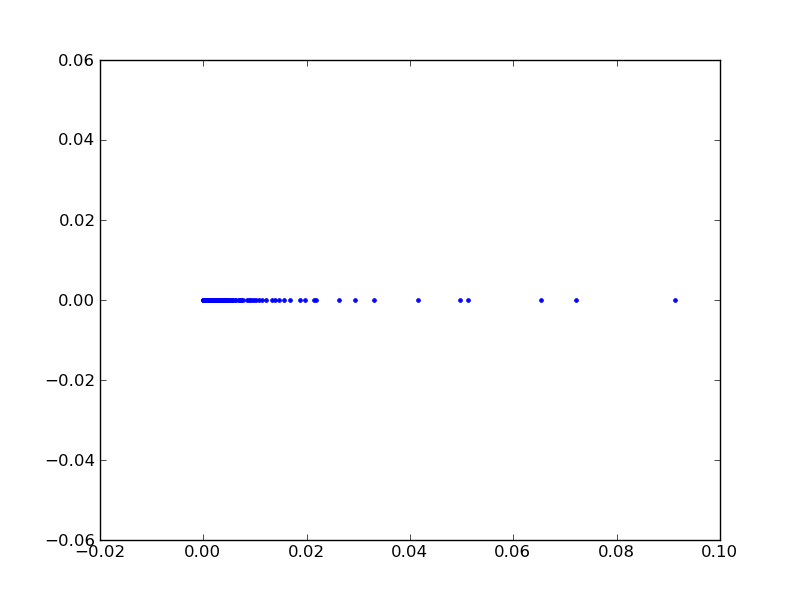
\includegraphics[width=4.0in]{img/wu2.png}
\end{figure}

To account for 90\% variance, we have to include 82 eigenvectors.
To account for 95\% variance, we have to include 136 eigenvectors.


\section*{WU3}
\begin{figure}[here]
	\center
	\caption{wu3}
	\label{fig:wu3}
	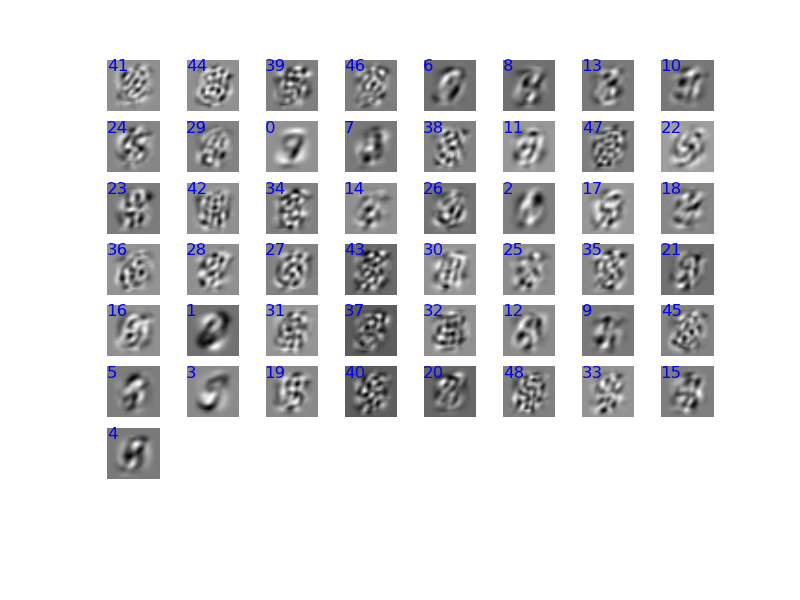
\includegraphics[width=6.0in]{img/wu3.png}
\end{figure}
No, they do not look like digits.